\section{Introduction}\label{sec:introduction}

The term Industry 4.0 (I. 4.0), as it was introduced by the German government in an effort to kick start a new paradigm in the manufacturing domain, describes a model towards enabling smart, flexible and predictive manufacturing, therefore optimising existing production processes and creating new business opportunities. \cite{i40gov} I. 4.0, also stated as the 4th Industrial Revolution\cite{revolution}, consists of four essential principles: interconnection between various devices (sensors, control units, machines, etc.) on the shop floor, information transparency to enable the creation of digital twins (virtual representations of objects), assistance for human operators and the use of Cyber-Physical-Systems (CPS) to enable smart manufacturing by applying decentralized decision making at the lower levels of production, therefore incorporating communication technologies, Internet of Things (IoT) and Machine Learning approaches. \cite{design}  

The implementation of the I. 4.0 concept is thus transforming the current automation pyramid \cite{autoPy} towards Smart Factories \cite{smartFac}, where not only the factories themselves, but where also the products are interconnected resulting in a decentralized/distributed ecosystem which is depicted in Fig. 1. The advantages of Smart Manufacturing over the traditional approach lie in the ability to analyse the running processes more efficiently as well as to apply reasoning to the data, which enables predictive manufacturing where machines can be controlled on a finer scale, resulting in individual maintenance scheduling on the shop floor and therefore in an improved production cycle.\cite{cpsAdv}

\begin{figure}
	\centering
	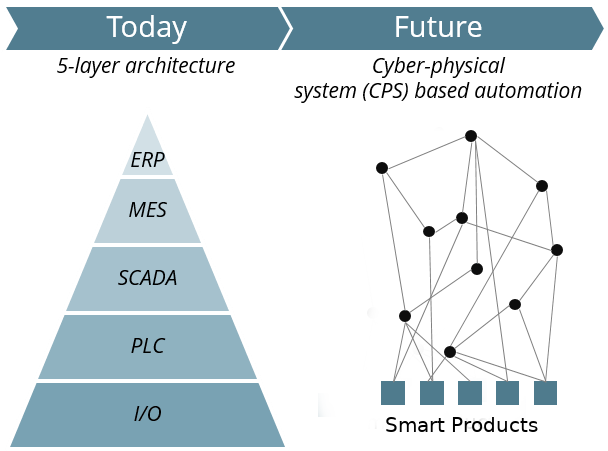
\includegraphics[scale=0.3]{comparison_autoHira_SF.png}
	\caption{Comparison between the traditional 5-layer automation Hierarchie and the future production architecture based on CPSs}
\end{figure}

However the implementation of the I.4.0 concept currently suffers from different drawbacks, as the manufacturing context applies different limitations on the integration. One of the key drawbacks lies in the latency requirements of factories. \cite{latency} Depending on the domain, it may be required to provide up to real time communication between devices as even small latencies can lead to delays of the production/assembly lines or even outages. Another problem arises from the amount of devices that gather data and therefore the amount of data that has to be processed. \cite{bigData} Even small devices can accumulate large sets of data over time, thus resulting in large datasets for the shop floor, as many thousand sensors and machines are part of the shop floor, and therefore requiring big data concepts. Given that most current implementations rely on a centralized cloud approach(a key enabler of automation), this creates a prominent data stream and therefore a heavy load towards the cloud, resulting in a bottleneck and leading to inefficient processing of the data. Another major concern is the power consumption of the sensing devices. \cite{fogDep} As sensing devices are usually constrainted and in certain use cases located in places difficult to reach efficiently, it is of importance to define communication methods that reduce the energy consumption of the devices, thus improving the battery lifetime.

Edge technologies introduce a way to tackle the above stated problems by improving the computational workflow. The term Edge refers to concepts where the processing of data is not achieved at a centralized node, but where the logic of the system is pushed to the edges of the network and thus closer to the devices. \cite{edgeDef} This concept is sometimes also referred to as FOG computing as these terms are not strictly defined and therefore used interchangeably. One way to differentiate these terms is depicted in Fig.2, where the Edge layer refers to the devices and the Fog layer represents a higher processing step. The addition of this processing step between the device layer and the cloud introduces a possibility to improve for example the latency of such systems.

\begin{figure}
	\centering
	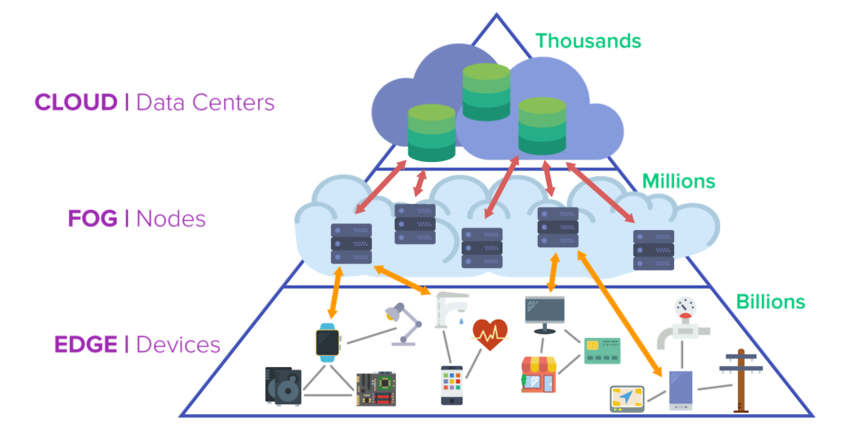
\includegraphics[scale=0.3]{edge_fog_cloud.png}
	\caption{Example of the division between Edge/Fog and the Cloud}
\end{figure}

This paper surveys the current trends in industrial edge computing, which leads towards smart manufacturing. It identifies key technologies, introduces concepts to integrate these technologies into existing production facilities as well as provides an overview on the benefits as well as drawbacks of these systems. This paper is therefore organized as follows. Section II provides an outline of related work on this topic. Section III introduces key technologies used for industrial edge computing, Section IV outlines integration concepts of these approaches and in Section V a discussion on the current state of industrial edge computing is provided. Section VI concludes this paper.

Cloud Computing and fog computing are rapidly replacing every section of the online or physical industry which involves processing data. Cloud computing charges only what you use so it is a pay as you store solution which is a massive achievement in the current era. One good aspect cloud computing provides is that you can replace the raw equipment cost directly into online scalable systems. On the other hand, a shortcome of Cloud Computing systems is observed where there is connectivity issues. Currently, this era belongs to online data stream processing with autonomous systems, and unreliability of network may be hazardous in such situations. Fog computing has given answers to many questions like how to store and transfer data to distributed systems without occupying the space and processing power at the server end in manufacturing support systems. Rather it has been transferred to the ‘edges', which means that all the space and time used to process data would be on the data producing edge node. 

\section{Initiatives and Future Engineering}\label{sec:future_engineering}


To help cope with the challenges that come, steps which are being taken are providing the opportunity to create new and innovative services to process data efficiently. Fog computing is helping resolve the issue of data flow and data diverse geo location by consuming the data at sites likes grid stations and devices. Collector at this step also processes data and provides commands to actuators also. Next is the reporting phase where machine shows visualizations to humans end machines. To perform all these steps fog computing systems have been observed to take seconds to minutes. Time scale increases if wider edge area is being considered but the impact on the cloud simultaneously decreases. Talking about manufacturing systems in this era, it is quite impressive to see growing role of integrated manufacturing information systems support manufacturing processes. In these systems integration has been done to reduce customer requirement mismatch. Modern trends have been introduced in the manufacturing support systems like internet of things, cloud computing for access to computing power, big data to analyze larger sets of structural and nonstructural data, automation in control systems. The concept of industry 4.0 in and smart manufacturing in Germany has led to revolution which other countries are also following. These are collectively called CPS which autonomously exchange information, trigger actions and control each other independently. Complete companies are now intelligence hubs covering the gap between digital and real world. Dynamic re-engineering processes are being introduced to respond flexibly to disruptions and failures. Two way horizontal integration is helping in cyber physical systems as well. CPPS are collected of autonomous components and modules which cooperate in a manner dependent on the situation in all stages of production. Starts from processes that are carried out by means of production devices and logistics network. CPPS systems open prospect for building applications in different areas. The implementation of CPPS systems is identified with industry revolution.

Due to criticality of the systems, and increasing amount of data to terabytes, the processing of data is gaining importance, especially where decision has to be made faster. Hence closer the control decisions to the process being monitored better it is. The decision records within the company help the security of data as well. Data transferring delay has been reduced also. In this paper further it is explained how fog computing addresses the needs of modern manufacturing enterprises. There are 5 parameters known as 5C to compute i.e. which consist of Connection (sensor and networks), Cloud (data on demand), Content (correlation and meaning), Community (sharing and social), and Customization (personalization and value). This opens door for implementation of CAx (computer aided systems) engineering software in “as a service” model. However it requires a lot of computational power. Another perspective that fog computing opens is the possibility to implement geo-distributed applications. Fog computing infrastructure allows access to the cloud and its computing everywhere and at the edge of the network. This makes a great viewpoint for solutions related to technical infrastructure monitoring which is related with the data acquisition from groups of sensors deployed on major areas. Further horizon is to implement geo distributed applications. Fog computing architecture allows access to cloud from every edge node. This makes a great perspective for solutions related to technical infrastructure monitoring which is associated with the data acquisition from groups of sensors deployed on major areas. Therefore from manufacturing perspective fog computing due to wide range of applications, has a high prospect of development in the field of production of support systems.
